\documentclass[10pt,aspectratio=169]{beamer}
\usepackage{../../common/foundationsmacro-beamer}
\usepackage{pgfplots}
\pgfplotsset{compat=1.18}
\usepgfplotslibrary{fillbetween}
\usepackage{tikz}
\usetikzlibrary{calc,arrows.meta,decorations.pathreplacing,patterns,shapes,positioning,intersections,math,backgrounds,plotmarks,matrix}
\usepackage{booktabs}
\usepackage{bm}

% Preserve the original diagram colors using the shared course palette.
\colorlet{TitleBlue}{MacroBlue}
\definecolor{darkgreen}{rgb}{0.0, 0.5, 0.0}
\definecolor{lightblue}{rgb}{0.3, 0.5, 0.55}
\definecolor{colormodel}{rgb}{0.3, 0.5, 0.55}
\definecolor{green2}{rgb}{0.4660, 0.6740, 0.1880}
\definecolor{red2}{rgb}{0.8500,0.3250,0.0980}
\colorlet{emphblue}{TitleBlue!25}

% Retain the original convention for leisure in mathematical expressions.
\AtBeginDocument{%
    \mathcode`l="8000
    \begingroup\lccode`\~=`\l%
    \lowercase{\endgroup\def~}{\ell}%
}

\title[Consumption and Saving]{Chapter V: Consumption and Saving}
\author[Bueren]{Jes\'{u}s Bueren}
\institute{}
\date{}

\begin{document}
\begin{frame}[plain]
    \titlepage
\end{frame}

\begin{frame}{Consumption and Saving}

\begin{itemize}
    \item Every day, people face a basic choice:
    \begin{itemize}
        \itemvso consume today
        \itemvso or save for the future
    \end{itemize}
    \vspace{0.3cm}

    \item Examples:
    \begin{itemize}
        \itemvso spend all your salary or save part of it?
        \itemvso buy a new phone now or put money aside?
    \end{itemize}
    \vspace{0.3cm}

    \item This chapter asks:
    \begin{itemize}
        \itemvso How do people decide how much to consume?
        \itemvso Why do people save?
        \itemvso How do income and interest rates affect these decisions?
    \end{itemize}
\end{itemize}

\end{frame}

\begin{frame}{A Simple Two-Period World}

\begin{itemize}
    \item Life is divided into two periods:
    \begin{itemize}
        \itemvso Period 1: today
        \itemvso Period 2: tomorrow
    \end{itemize}
    \vspace{0.3cm}

    \item You receive income in each period
    \begin{itemize}
        \itemvso \(y_1\) today
        \itemvso \(y_2\) tomorrow
    \end{itemize}
    \vspace{0.3cm}

    \item You choose how much to:
    \begin{itemize}
        \itemvso consume today (\(c_1\))
        \itemvso consume tomorrow (\(c_2\))
    \end{itemize}
   
\end{itemize}

\end{frame}

\begin{frame}{A Savings Technology}

\begin{itemize}
    \item You have access to a simple way to save money
    \begin{itemize}
        \itemvso think of a bank account
    \end{itemize}
    \vspace{0.3cm}

    \item In period 1, you can save part of your income \(y_1\)
    \begin{itemize}
        \itemvso let \(s\) be the amount you save
    \end{itemize}
    \vspace{0.3cm}

    \item In period 2, your savings grow
    \begin{itemize}
        \itemvso saving \(s\) today gives \( (1+R)s \) tomorrow
    \end{itemize}
    \vspace{0.3cm}

    \item \(R\) is the \textbf{interest rate}
\end{itemize}

\end{frame}

\begin{frame}{Saving and Borrowing}

\begin{itemize}
    \item Let \(s\) be savings in period 1
    \begin{itemize}
        \itemvso \(s > 0\): savings
        \itemvso \(s < 0\): borrowing
    \end{itemize}
    \vspace{0.3cm}

    \item In period 2:
    \begin{itemize}
        \itemvso saving or borrowing changes resources by \((1+R)s\)
    \end{itemize}

    \itemvso Same interest rate for both
\end{itemize}
\end{frame}

\begin{frame}{The Consumption--Saving Model}

\begin{itemize}
    \item Budget constraints in each period:
    \vspace{0.3cm}
    \itemvso Period 1 (today):
    \[
    c_1 + s = y_1
    \]
    \item Period 2 (tomorrow):
    \[
    c_2 = y_2 + (1+R)s
    \]
\end{itemize}

\end{frame}


\begin{frame}{Limits on Saving and Borrowing}

\begin{itemize}
    \item How much can you save?
    \begin{itemize}
        \itemvso you cannot save more than your income today
        \[
        s \le y_1
        \]
    \end{itemize}
    \item How much can you borrow?
    \begin{itemize}
        \itemvso you must be able to repay tomorrow
        \[
        (1+R)s \ge -\,y_2
        \]
        \item[] which implies:
        \[
        s \ge -\,\frac{y_2}{1+R}
        \]
    \end{itemize}
\end{itemize}

\end{frame}


\begin{frame}{Utility Function}

\begin{itemize}
    \item Preferences describe how people value consumption
    \vspace{0.3cm}

    \item In general, utility depends on consumption in both periods:
    \[
    W(c_1, c_2)
    \]
    \vspace{-0.3cm}

    \item We will use a simple and common specification:
    \[
    W(c_1, c_2)=U(c_1) + \beta\, U(c_2)
    \]
    \vspace{-0.3cm}

    \item Utility today plus discounted utility tomorrow
\end{itemize}

\end{frame}

\begin{frame}{The Discount Factor}

\begin{itemize}
    \item \( \beta \) is the \textbf{subjective discount factor}
    \vspace{0.3cm}

    \item It measures how much weight you place on future consumption
    \vspace{0.3cm}
    \begin{itemize}
        \item Higher \( \beta \): more patient
        \item Lower \( \beta \): more impatient
    \end{itemize}
    \vspace{0.3cm}

    \item If \( \beta < 1 \):
    \begin{itemize}
        \item future consumption is discounted
    \end{itemize}
    \vspace{0.3cm}

    \item If one period is one year, a typical value is:
    \[
    \beta \approx 0.98
    \]
\end{itemize}

\end{frame}

\begin{frame}{The Consumption--Saving Model}

\begin{itemize}
    \item The student chooses consumption to maximize:
    \[
    \max_{c_1, c_2,s}U(c_1) + \beta\, U(c_2)
    \]
    \vspace{-0.3cm}

    \item Subject to:
    \[
    c_1 + s = y_1
    \]
    \[
    c_2 = y_2 + (1+R)s
    \]
    \vspace{-0.2cm}

    \item And limits on saving and borrowing
\end{itemize}

\end{frame}

\begin{frame}{Solving the Model: Step 1}

\begin{itemize}
    \item Combine the two budget constraints into one
    \vspace{0.3cm}

    \item Intertemporal budget constraint:
    \[
    c_1 + \frac{1}{1+R} c_2
    =
    y_1 + \frac{1}{1+R} y_2
    \]
    \vspace{-0.3cm}

    \item This eliminates saving \(s\) from the problem
    \vspace{0.3cm}

    \item Interpretation:
    \begin{itemize}
        \itemvso present value of consumption
        \itemvso equals present value of income
    \end{itemize}
\end{itemize}

\end{frame}

\begin{frame}{Present Value}

\begin{itemize}
    \item Question:
    \begin{itemize}
        \item how much does it cost \textbf{today} to get 1 unit of consumption tomorrow?
    \end{itemize}
    \vspace{0.3cm}

    \item If you save 1 unit today, tomorrow you get:
    \[
    1+R
    \]
    \vspace{0.3cm}

    \item Therefore, to get 1 unit tomorrow, you must save today:
    \[
    \frac{1}{1+R}
    \]
    \vspace{0.3cm}

    \item This is the \textbf{present value} of one unit of future consumption
\end{itemize}

\end{frame}
\begin{frame}{Understanding Present Value}

\begin{itemize}
    \item Imagine you want to buy a surfboard next year for €500
    \vspace{0.2cm}
    
    \item How much do you need to save today if the bank pays interest \(R\)?
    \[
    \text{Today’s cost} = \frac{500}{1+R}
    \]  
    \item Example:
    \begin{itemize}
        \itemvso If \(R = 0.05\) (5\% interest)
        \itemvso To get €500 next year, you save:
        \[
        \frac{500}{1.05} \approx 476.19 \text{ euros today}
        \]
    \end{itemize}
    \textit{If you want to buy that surfboard next year, you only need €476 today if you put it in the bank at 5\%}
    
    \itemvso Present value computes the price today of future consumption: Buying a surf board for period 2 is cheaper than buying it today.
\end{itemize}

\end{frame}



\begin{frame}{Solving the Model: Step 2}

\begin{itemize}
    \item Use the intertemporal budget constraint to eliminate \(c_2\)
    \vspace{0.3cm}

    \item From the budget constraint:
    \[
    c_2 = (1+R)\big(y_1 + \frac{y_2}{1+R} - c_1\big)
    \]
    \item Plug into utility:
    \[
    U(c_1) + \beta U(c_2)
    \]
    \item Now the problem has:
    \begin{itemize}
        \itemvso one choice variable: \(c_1\)
    \end{itemize}
\end{itemize}

\end{frame}


\begin{frame}{Solving the Model: Step 3}

\begin{itemize}
    \item The household chooses \(c_1\) to maximize:
    \[
    U(c_1)
    +
    \beta U\!\left(
    (1+R)\left[y_1 + \frac{y_2}{1+R} - c_1\right]
    \right)
    \]
    \vspace{0.3cm}

    \item Take the derivative with respect to \(c_1\)
    \vspace{0.3cm}

    \item Set it equal to zero (first-order condition)
\end{itemize}

\end{frame}

\begin{frame}{The Consumption Euler Equation}

\begin{itemize}
    \item First-order condition:
    \[
    U'(c_1)
    =
    \beta (1+R) U'(c_2)
    \]
    \vspace{0.3cm}

    \item This is called the \textbf{Euler equation}
    \vspace{0.3cm}
    \begin{itemize}
        \item marginal utility today
        \item equals discounted, interest-adjusted marginal utility tomorrow
    \end{itemize}
\end{itemize}

\end{frame}

\begin{frame}{Euler Equation: Variational Argument}

\begin{itemize}
    \item Start from a candidate optimal choice \((c_1, c_2)\)
    \vspace{0.2cm}
    
    \item Suppose the student considers saving a tiny bit more today
    \vspace{0.2cm}
    
    \item Marginal cost (today):
    \[
    U'(c_1)
    \]
    
    \item Marginal benefit (tomorrow):
    \[
    \beta (1+R) U'(c_2)
    \]
    
    \item Optimal choice requires:
    \[
    U'(c_1) = \beta (1+R) U'(c_2)
    \]
    
    \item This is the \textbf{consumption Euler equation}
\end{itemize}

\end{frame}


\begin{frame}{The Budget Constraint}
\begin{center}
\begin{tikzpicture}
    \begin{axis}[
        axis lines=middle,
        xlabel={$c_1$},
        ylabel={$c_2$},
        xlabel style={font=\small\itshape, at={(axis description cs:1.02,0.055)}, anchor=south west},
        ylabel style={font=\small\itshape, at={(axis description cs:0.02,0.98)}, anchor=south west, rotate=0, fill=white, inner sep=1pt},
        xmin=0, xmax=12.5,
        ymin=-2.6, ymax=13.5,
        width=10cm,
        height=7.5cm,
        samples=200,
        domain=0:10,
        xtick=\empty,
        ytick=\empty,
        axis line style={black, thin},
        clip=true,
    ]

    % Intertemporal budget line: c2 = (1+R)y1 + y2 - (1+R)c1
    % Example values only determine the picture's scale.
    \pgfmathsetmacro{\R}{0.2}
    \pgfmathsetmacro{\yone}{4}
    \pgfmathsetmacro{\ytwo}{6}
    \pgfmathsetmacro{\cOneInt}{\yone + \ytwo/(1+\R)}
    \pgfmathsetmacro{\cTwoInt}{(1+\R)*\yone + \ytwo}
    \pgfmathsetmacro{\labelBand}{-1.1}

    % Feasible set
    \addplot[draw=none, fill=emphblue, fill opacity=0.35]
        coordinates {(0,0) (0,\cTwoInt) (\cOneInt,0)} \closedcycle;

    % Saving and borrowing regions below the c1 axis
    \addplot[draw=none, fill=green2!22, fill opacity=0.95]
        coordinates {(0,\labelBand) (0,0) (\yone,0) (\yone,\labelBand)} \closedcycle;
    \addplot[draw=none, fill=red2!22, fill opacity=0.95]
        coordinates {(\yone,\labelBand) (\yone,0) (\cOneInt,0) (\cOneInt,\labelBand)} \closedcycle;

    % Budget frontier
    \addplot[color=red!80!black, line width=2pt] {\cTwoInt - (1+\R)*x};
    \draw[-{Latex[length=2.2mm]}, red!80!black, thick]
        (axis cs:8.9,11.1) -- (axis cs:4.8,5.04);
    \node[font=\small, color=red!80!black, fill=white, inner sep=1.5pt, align=left]
        at (axis cs:9.25,11.45) {$c_2=(1+R)\big(y_1+\frac{y_2}{1+R}-c_1\big)$};

    % Intercepts
    \addplot[only marks, mark=*, color=red!80!black, mark size=2.5pt]
        coordinates {(0,\cTwoInt) (\cOneInt,0)};
    \node[font=\small, anchor=west, color=red!80!black]
        at (axis cs:0.15,\cTwoInt) {$\left(0,\,(1+R)y_1+y_2\right)$};
    \node[font=\small, anchor=south west, color=red!80!black]
        at (axis cs:\cOneInt,0) {$\left(y_1+\frac{y_2}{1+R},\,0\right)$};

    % Endowment point
    \addplot[only marks, mark=*, black, mark size=2.5pt] coordinates {(\yone,\ytwo)};
    \node[font=\small, anchor=south west] at (axis cs:\yone,\ytwo) {$\left(y_1,y_2\right)$};
    \draw[gray, densely dashed] (axis cs:\yone,\labelBand) -- (axis cs:\yone,\ytwo);
    \draw[gray, densely dashed] (axis cs:0,\ytwo) -- (axis cs:\yone,\ytwo);

    % Slope marker
    \draw[red!80!black, line width=0.9pt] (axis cs:5.1,2.5) -- (axis cs:6.8,2.5);
    \node[font=\small, color=red!80!black] at (axis cs:5.3,3.1) {$1+R$};

    % Braces highlighting the saving and borrowing regions
    \draw[decorate, decoration={brace, mirror, amplitude=5pt}, thick, darkgreen]
        (axis cs:0.15,-0.18) -- (axis cs:\yone-0.15,-0.18)
        node[midway, below=6pt, font=\small, color=darkgreen] {Saving $(s>0)$};
    \draw[decorate, decoration={brace, mirror, amplitude=5pt}, thick, red2]
        (axis cs:\yone+0.15,-0.18) -- (axis cs:\cOneInt-0.15,-0.18)
        node[midway, below=6pt, font=\small, color=red2] {Borrowing $(s<0)$};

    \end{axis}
\end{tikzpicture}
\end{center}
\end{frame}

\begin{frame}{Preferences over Consumption}
\begin{center}
\begin{tikzpicture}
    \begin{axis}[
        axis x line=middle,
        axis y line=left,
        xlabel={},
        ylabel={},
        xmin=0, xmax=10.2,
        ymin=-0.8, ymax=11.8,
        width=10cm,
        height=7.1cm,
        samples=400,
        domain=0.7:10,
        xtick=\empty,
        ytick=\empty,
        axis line style={black, thin, -{Latex[length=2mm]}},
        clip=false,
    ]

    % Smooth indifference curves, styled to match the WorkLeisure figure
    \addplot[color=blue!70!black, line width=2pt, smooth] {16/(x+1.3) + 3.0};
    \addplot[color=blue!65!black, line width=2pt, smooth] {12/(x+1.3) + 1.9};
    \addplot[color=blue!60!black, line width=2pt, smooth] {8/(x+1.3) + 0.8};

    \node[font=\small\itshape, fill=white, inner sep=1pt, anchor=west]
        at (axis cs:10.18,0) {$c_1$};
    \node[font=\small\itshape, fill=white, inner sep=1pt, anchor=south]
        at (axis cs:0,11.78) {$c_2$};
    \node[font=\small\bfseries, color=blue!70!black, right, fill=white, inner sep=1pt] at (axis cs:8.7,4.55) {$W_3$};
    \node[font=\small\bfseries, color=blue!65!black, right, fill=white, inner sep=1pt] at (axis cs:8.7,3.15) {$W_2$};
    \node[font=\small\bfseries, color=blue!60!black, right, fill=white, inner sep=1pt] at (axis cs:8.7,1.75) {$W_1$};

    \end{axis}
\end{tikzpicture}
\end{center}
\end{frame}

\begin{frame}{Preferences over Consumption: More Impatient Household}
\begin{center}
\begin{tikzpicture}
    \begin{axis}[
        axis x line=middle,
        axis y line=left,
        xlabel={},
        ylabel={},
        xmin=0, xmax=10.2,
        ymin=0.0, ymax=11.8,
        width=10cm,
        height=7.1cm,
        samples=400,
        domain=0.7:10,
        xtick=\empty,
        ytick=\empty,
        axis line style={black, thin, -{Latex[length=2mm]}},
        clip=false,
    ]

    % Baseline high-beta preferences
    \addplot[color=blue!70!black, line width=2pt, smooth] {16/(x+1.3) + 3.0};
    \addplot[color=blue!65!black, line width=2pt, smooth] {12/(x+1.3) + 1.9};
    \addplot[color=blue!60!black, line width=2pt, smooth] {8/(x+1.3) + 0.8};

    % Lower beta makes indifference curves steeper in (c1,c2) space
    \addplot[color=blue!70!black, line width=1.8pt, dashed, smooth] {15/(x+1.0) + 2.2};
    \addplot[color=blue!65!black, line width=1.8pt, dashed, smooth] {11/(x+1.0) + 1.3};
    \addplot[color=blue!60!black, line width=1.8pt, dashed, smooth] {7.5/(x+1.0) + 0.6};

    \node[font=\small\itshape, fill=white, inner sep=1pt, anchor=west]
        at (axis cs:10.18,0) {$c_1$};
    \node[font=\small\itshape, fill=white, inner sep=1pt, anchor=south]
        at (axis cs:0,11.78) {$c_2$};
    \node[font=\small\bfseries, color=blue!70!black, right, fill=white, inner sep=1pt] at (axis cs:8.7,4.55) {$W_3$};
    \node[font=\small\bfseries, color=blue!65!black, right, fill=white, inner sep=1pt] at (axis cs:8.7,3.15) {$W_2$};
    \node[font=\small\bfseries, color=blue!60!black, right, fill=white, inner sep=1pt] at (axis cs:8.7,1.75) {$W_1$};
    \node[font=\small, align=left, fill=white, inner sep=1.5pt] at (axis cs:2.9,9.25) {solid: high $\beta$\\dashed: low $\beta$};

    \end{axis}
\end{tikzpicture}
\end{center}
\end{frame}

\begin{frame}{Optimal Choice}
\begin{center}
\begin{tikzpicture}
    \begin{axis}[
        axis lines=left,
        xlabel={},
        ylabel={},
        xmin=0, xmax=10.2,
        ymin=0.0, ymax=11.8,
        width=10cm,
        height=7.1cm,
        samples=400,
        xtick=\empty,
        ytick=\empty,
        axis line style={black, thin, -{Latex[length=2mm]}},
        clip=false,
    ]

    % Parameters
    \pgfmathsetmacro{\R}{0.2}
    \pgfmathsetmacro{\yone}{4}
    \pgfmathsetmacro{\ytwo}{6}
    \pgfmathsetmacro{\betaopt}{0.8}
    \pgfmathsetmacro{\cOneInt}{\yone + \ytwo/(1+\R)}
    \pgfmathsetmacro{\cTwoInt}{(1+\R)*\yone + \ytwo}
    \pgfmathsetmacro{\cOnestar}{5}
    \pgfmathsetmacro{\cTwostar}{4.8}
    \pgfmathsetmacro{\kopt}{ln(\cOnestar) + \betaopt*ln(\cTwostar)}

    % Budget set and frontier
    \addplot[draw=TitleBlue!45, line width=0.8pt, fill=emphblue, fill opacity=0.20]
        coordinates {(0,0) (0,\cTwoInt) (\cOneInt,0)} \closedcycle;
    \addplot[color=red!80!black, line width=2pt, domain=0:\cOneInt] {\cTwoInt - (1+\R)*x};

    % Indifference curve tangent at the optimum
    \addplot[color=blue!70!black, line width=2pt, smooth, domain=2.5:9.1]
        {exp((\kopt - ln(x))/\betaopt)};

    % Endowment point and guides
    \addplot[only marks, mark=*, mark size=2.5pt, color=black]
        coordinates {(\yone,\ytwo)};
    \node[font=\small, anchor=south east] at (axis cs:\yone,\ytwo) {$\left(y_1,y_2\right)$};
    \draw[gray, densely dashed] (axis cs:\yone,0) -- (axis cs:\yone,\ytwo);
    \draw[gray, densely dashed] (axis cs:0,\ytwo) -- (axis cs:\yone,\ytwo);
    \node[font=\small, anchor=north] at (axis cs:\yone,0) {$y_1$};
    \node[font=\small, anchor=east] at (axis cs:0,\ytwo) {$y_2$};

    % Optimal choice
    \addplot[only marks, mark=*, mark size=2.8pt, color=black]
        coordinates {(\cOnestar,\cTwostar)};
    \node[font=\small, anchor=south west] at (axis cs:\cOnestar,\cTwostar) {$\left(c_1^*,c_2^*\right)$};

    % Guides to the axes
    \draw[gray, densely dashed] (axis cs:\cOnestar,0) -- (axis cs:\cOnestar,\cTwostar);
    \draw[gray, densely dashed] (axis cs:0,\cTwostar) -- (axis cs:\cOnestar,\cTwostar);
    \node[font=\small, anchor=north] at (axis cs:\cOnestar,0) {$c_1^*$};
    \node[font=\small, anchor=east] at (axis cs:0,\cTwostar) {$c_2^*$};

    % Labels
    \node[font=\small\itshape, fill=white, inner sep=1pt, anchor=west]
        at (axis cs:10.18,0) {$c_1$};
    \node[font=\small\itshape, fill=white, inner sep=1pt, anchor=south]
        at (axis cs:0,11.78) {$c_2$};

    \end{axis}
\end{tikzpicture}
\end{center}
\end{frame}

\begin{frame}{An Increase in the Interest Rate}

\begin{itemize}
    \item When \(R\) increases, the budget line becomes \textbf{steeper} around the endowment point \((y_1,y_2)\)

    \itemvso \textbf{Substitution effect:}
    \begin{itemize}
        \item future consumption becomes cheaper relative to current consumption
        \item households want to shift consumption from period 1 to period 2
        \item therefore: lower \(c_1\), higher \(c_2\)
    \end{itemize}

    \itemvso \textbf{Income effect:} depends on whether the household is a saver or a borrower
    \begin{itemize}
        \item if the household is a \textbf{saver} (\(s>0\)), higher \(R\) raises lifetime resources
        \item if the household is a \textbf{borrower} (\(s<0\)), higher \(R\) lowers lifetime resources
    \end{itemize}

    \itemvso Therefore:
    \begin{itemize}
        \item \textbf{Saver:} income effect raises both \(c_1\) and \(c_2\)
        \item \textbf{Borrower:} income effect lowers both \(c_1\) and \(c_2\)
        \item total effect on \(c_1\) is ambiguous for savers, while total effect on \(c_2\) is ambiguous for borrowers
    \end{itemize}
\end{itemize}

\end{frame}

\begin{frame}{Higher Interest Rate: Saver vs Borrower}
\centering
\begin{tikzpicture}[scale=0.92, every node/.style={font=\footnotesize}]

% --- LEFT PANEL: SAVER ---
\begin{scope}[shift={(0,0)}]
    \node at (2.8,5.9) {\textbf{Saver}};

    % Axes
    \draw[->, thick] (0,0) -- (5.7,0) node[below] {$c_1$};
    \draw[->, thick] (0,0) -- (0,5.8) node[left] {$c_2$};

    % Endowment
    \coordinate (yS) at (3.3,1.1);
    \filldraw[black] (yS) circle (2.1pt);
    \draw[densely dashed, gray] (yS) -- (3.3,0) node[below] {$y_1$};
    \draw[densely dashed, gray] (yS) -- (0,1.1) node[left] {$y_2$};

    % Budget constraints
    \draw[red!70!black, line width=2pt] (0,4.4) -- (4.4,0);
    \draw[red!40!orange, line width=2pt, dashed] (0.689,5.8) -- (3.911,0);
    \draw[gray!80, line width=1.4pt, dotted] (0,5.90) -- (3.278,0);

    % Indifference curves
    \draw[color=blue!65!black, line width=2pt, domain=1.0:4.2, smooth] plot (\x, {4.84/\x});
    \draw[color=blue!40!cyan, line width=2pt, domain=1.15:4.2, smooth] plot (\x, {6.89/\x});
    \node[color=blue!65!black, fill=white, inner sep=1pt] at (3.95,1.55) {$W_1$};
    \node[color=blue!40!cyan, fill=white, inner sep=1pt] at (3.55,2.15) {$W_2$};

    % Points A, S, B
    \coordinate (A) at (2.2,2.2);
    \coordinate (S) at (1.64,2.95);
    \coordinate (B) at (1.96,3.52);

    \filldraw[blue!65!black] (A) circle (2.1pt);
    \node[anchor=south west] at (A) {$A$};

    \filldraw[gray!80!black] (S) circle (2.1pt);
    \node[anchor=north east] at (S) {$S$};

    \filldraw[blue!40!cyan] (B) circle (2.1pt);
    \node[anchor=south west] at (B) {$B$};
\end{scope}

% --- RIGHT PANEL: BORROWER ---
\begin{scope}[shift={(7.0,0)}]
    \node at (2.8,5.9) {\textbf{Borrower}};

    % Axes
    \draw[->, thick] (0,0) -- (5.7,0) node[below] {$c_1$};
    \draw[->, thick] (0,0) -- (0,5.8) node[left] {$c_2$};

    % Endowment
    \coordinate (yB) at (0.7,3.3);
    \filldraw[black] (yB) circle (2.1pt);
    \draw[densely dashed, gray] (yB) -- (0.7,0) node[below] {$y_1$};
    \draw[densely dashed, gray] (yB) -- (0,3.3) node[left] {$y_2$};

    % Budget constraints
    \draw[red!70!black, line width=2pt] (0,4.0) -- (4.0,0);
    \draw[red!40!orange, line width=2pt, dashed] (0,5.4) -- (1.8,0);
    \draw[gray!80, line width=1.4pt, dotted] (0.376,5.8) -- (2.31,0);

    % Indifference curves
    \draw[color=blue!65!black, line width=2pt, domain=0.9:4.0, smooth] plot (\x, {4.0/\x});
    \draw[color=blue!40!cyan, line width=2pt, domain=0.65:3.0, smooth] plot (\x, {2.43/\x});
    \node[color=blue!65!black] at (3.75,1.55) {$W_1$};
    \node[color=blue!40!cyan] at (2.65,1.02) {$W_2$};

    % Points A, S, B
    \coordinate (A) at (2.0,2.0);
    \coordinate (S) at (1.155,3.464);
    \coordinate (B) at (0.9,2.7);

    \filldraw[blue!65!black] (A) circle (2.1pt);
    \node[anchor=south west] at (A) {$A$};

    \filldraw[gray!80!black] (S) circle (2.1pt);
    \node[anchor=south east] at (S) {$S$};

    \filldraw[blue!40!cyan] (B) circle (2.1pt);
    \node[anchor=north east] at (B) {$B$};
\end{scope}

\end{tikzpicture}
\end{frame}

\begin{frame}{Euler Equation with Log Utility}

\begin{itemize}
    \item Assume:
    \[
    U(c) = \log c \quad \Rightarrow \quad U'(c) = \frac{1}{c}
    \]
    \itemvso Total utility is given by:
    \[
    W(c_1,c_2)=U(c_1)+\beta U(c_2)=\log(c_1) + \beta \log(c_2)
    \]
    \itemvso The max of $W$ is found when Euler equation holds:
    \[
    \frac{1}{c_1} = \frac{\beta (1+R)}{c_2} \quad \Rightarrow \quad c_2 = \beta(1+R) c_1
    \]
    \item The Euler equation implies that consumption grows by factor \(\beta(1+R)\)

\end{itemize}

\end{frame}

\begin{frame}{Consumption Growth}

\begin{itemize}
    \item With log utility:
    \[
    \frac{c_2}{c_1} = \beta (1+R)
    \]
    \vspace{0.3cm}
    
    \item Notice:
    \begin{itemize}
        \item Consumption growth does NOT depend on income growth: \(y_1/y_2\)
        \item Whether you earn most of your income in period 1 or period 2, consumption grows at the same rate
    \end{itemize}
    
\end{itemize}

\end{frame}

\begin{frame}{Consumption-Savings: Why Not Just Track Income?}

\begin{itemize}
    \item Suppose most of your income comes in period 2
    \vspace{0.2cm}
    
    \item You could let consumption follow income:
    \[
    c_1 = y_1, \quad c_2 = y_2
    \]
    
    \item But this is not optimal because of diminishing marginal utility:
    \begin{itemize}
        \item Marginal utility is higher in period 1 (less consumption)
        \item Marginal utility is lower in period 2 (lots of consumption)
    \end{itemize}
    
    \itemvso By transferring some consumption to period 1, total utility increases
\end{itemize}

\end{frame}

\begin{frame}{Consumption Smoothing}

\begin{itemize}
    \item Assume:
    \[
    \beta(1+R) = 1
    \]
    
    \item Then the Euler equation implies:
    \[
    c_1 = c_2
    \]
    
    \item Interpretation:
    \begin{itemize}
        \item Optimal consumption does not depend on the timing of income
        \item Even if \(y_1\) is small and \(y_2\) is large, consumption is smoothed
        \item This is because of diminishing marginal utility
    \end{itemize}
\end{itemize}

\end{frame}

\begin{frame}{Consumption Growth and the Interest Rate}

\begin{itemize}
    \item Euler equation (log utility):
    \[
    \frac{c_2}{c_1} = \beta (1+R)
    \]
    
    \item Holding \(\beta\) fixed:
    \begin{itemize}
        \item Higher \(R\) → higher growth rate of consumption
        \item Why? Higher return on saving makes future consumption cheaper
        \item You save more today → consumes less today, more tomorrow
    \end{itemize}
    
\end{itemize}

\end{frame}




\begin{frame}{Solving for Consumption Levels}

\begin{itemize}
    \item With log utility, we have two equations:
   \begin{align*}
   \frac{c_2}{c_1} &= \beta (1+R) \\
    c_1 + \frac{1}{1+R} c_2 &= y_1 + \frac{1}{1+R} y_2
   \end{align*}   
    \item Unknowns: \(c_1\) and \(c_2\)
    \vspace{0.2cm}
    
    \item Solve these two equations to get the level of consumption in each period
\end{itemize}

\end{frame}

\begin{frame}{Level of Consumption: Solution}

\begin{itemize}
    \item Solving the system yields:
    \[
    c_1 = \frac{1}{1 + \beta} \left( y_1 + \frac{y_2}{1+R} \right)
    \]
    
        \item Consumption at time 1 is a fraction of the present value of lifetime income
        \itemvso Current income only matters insofar as it affects the present value
        \itemvso Current income is not special: consumption smooths over both periods
        \itemvso Permanent income hypothesis: what matters is life-time income and not any one period's
income.
\itemvso Two individuals $A$ and $B$ with $y^A_1 \neq y^B_1$ and $y^A_2 \neq y^B_2$ but with $y^A_1 + \frac{y^A_2}{1+R}=y^B_1 + \frac{y^B_2}{1+R}$  should consume the same
\end{itemize}
\end{frame}

\begin{frame}{Marginal Propensity to Consume (MPC)}
\begin{center}
\Large
Suppose you receive a surprise scholarship of \textbf{€1000}.\\[0.5cm]

\textbf{Question:} How much would you spend within a year, and how much would you save for later?
\end{center}

\pause
\begin{itemize}
    \item Think about whether you expect this scholarship to be a one-time bonus or a permanent increase in your income.
    \item How does that affect your decision to spend now versus later?
\end{itemize}
\end{frame}

\begin{frame}{Marginal Propensity to Consume out of transitory shock}

\begin{itemize}
    \item Suppose the agent income $y_1$ increases by a small amount, but the agent does \textbf{not} change its expectation of future income $y_2$
  \itemvso  This is perceived as a \textbf{transitory increase} (e.g., a one-time bonus).

    \itemvso How much does consumption respond? The answer is given by the \textbf{marginal propensity to consume} to a transitory shock
    
    \itemvso In our example with log utility:
    \[
    \text{MPC}_t = \frac{\partial c_1}{\partial y_1} = \frac{1}{1 + \beta} < 1
    \]
\itemvso The more impatient you are, the more you consume out of a transitory income shock
\end{itemize}
\end{frame}

\begin{frame}{Marginal Propensity to Consume out of permanent shock}

\begin{itemize}
    \item Suppose the agent income $y_1$ and $y_2$ increases by a small amount $\Delta$
  \itemvso  This is perceived as a \textbf{permanent increase} (e.g., a promotion).

    \itemvso How much does consumption respond? The answer is given by the \textbf{marginal propensity to consume} to a permanent shock
    
    \itemvso In our example with log utility:
    \[
    \text{MPC}_p = \frac{\partial c_1}{\partial \Delta} = \frac{1}{1 + \beta} + \frac{1}{1 + \beta}\frac{1}{1 + R} >   \frac{1}{1 + \beta}
    \]

\itemvso In the case $\beta(1+R)=1$ the $MPC_p=1$: your consumption increases one for one with your income.
\end{itemize}
\end{frame}

\begin{frame}{Does the Model fit the data?}
\begin{center}
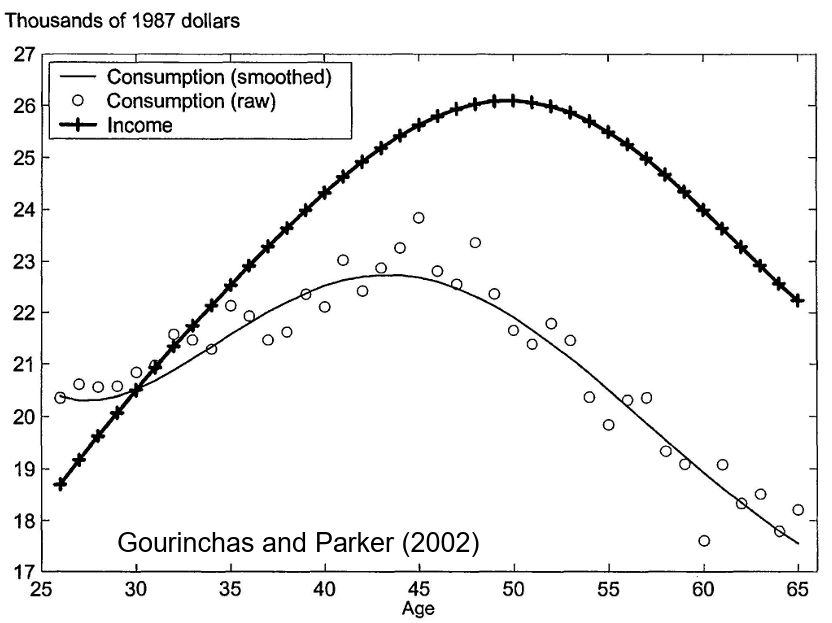
\includegraphics[scale=0.6]{figures/c-y.png}
\end{center}

\end{frame}

\begin{frame}{Does the Model fit the data?}
\begin{itemize}
    \item \textbf{Answer:} No
    

        \itemvso The model implies a \textbf{constant growth rate of consumption} (from the Euler equation)
        \itemvso Empirical data show a \textbf{hump-shaped pattern of consumption} over the life cycle
        \itemvso Observed consumption profiles \textbf{track income patterns}, whereas the model predicts consumption should be smooth
    
    \itemvso This highlights the need for more realistic features:  uncertainty, borrowing constraints, and life-cycle considerations.
    \itemvso $\beta(1+R)<1$ and credit constraints can replicate the pattern
\end{itemize}

\end{frame}

\begin{frame}{Key Takeaways: Consumption-Saving}
\begin{itemize}
    \item \textbf{Consumption Smoothing:} 
    \begin{itemize}
        \itemvso Diminishing marginal utility implies households should \textbf{borrow when income is low} and \textbf{save when income is high}.
    \end{itemize}

    \itemvso \textbf{Borrowing Constraints:} 
    \begin{itemize}
        \itemvso Limits on borrowing prevent households from smoothing consumption as much as they would like.
    \end{itemize}
\end{itemize}
\end{frame}


\end{document}
